\chapter{Numerik von gewöhnlichen Differentialgleichungen}

Der Inhalt dieses Kapitels ist größtenteils dem Buch von \cite{deuflhard_bornemann:2008} entnommen.


Gewöhnliche Differentialgleichung:
\begin{equation*}
 x'_i=f_i (t,x_1,\ldots,x_d ), \quad i=1,\ldots,d
\end{equation*}
wobei $(t,x) \in \R \times \R^d$ und $f_i \colon \Omega \to \R^d$, $\Omega \subseteq \R \times \R^d$ offen.

\begin{itemize}[nolistsep]
	\item Die Variable $t$ ist häufig als Zeit interpretierbar, man spricht daher häufig von \emph{Evolutionsproblemen}.
	\item $x$ heißt \emph{Zustandsvektor}.
	\item $\R^d$ mit $x \in \R^d$ heißt \emph{Zustandsraum}.
	\item $\R \times \R^d$ heißt \emph{erweiterter Zustandsraum}.
\end{itemize}

\paragraph{Beispiele}
\begin{enumerate}
 \item (Radioaktiver Zerfall) Finde $x : \R \to \R$ so dass $x' =-kx$. \\
   \emph{Achtung:} Traditionell verwendet man das gleiche Symbol für Zustände $x \in \R^d$ und Funktionen in den Zustandsraum $x : \R \to \R^d$.  Nicht verwirren lassen!
 %
 \item (Zwei-Massen-Schwinger) $d=4$
  \begin{align*}
	x'_1 & =x_3 \\
	x'_2 & =x_4 \\
	x'_3 & =\frac{1}{m_1} \big(-k_1x_1+k_2 (x_2-x_1) \big) \\
	x'_4 & =\frac{1}{m_2} \big(k_2 (x_1-x_2)-k_3x_2 \big)
  \end{align*}
  Dürfen denn keine höheren Ableitungen vorkommen?

 \item (Zwei-Massen-Schwinger physikalisch).

   \begin{tikzpicture}
    % left fixture
    \node[rectangle,pattern=north east lines,minimum width=1cm,minimum height=2cm] (l) at (-5,0) {};
    \draw[thick] (-4.5, 1) -- (-4.5, -1);
    % left mass
    \node[circle,fill=magenta,inner sep=2.5mm] (a) at (-2,0) {$m_1$};
    % right mass
    \node[circle,fill=magenta,inner sep=2.5mm] (b) at (+2,0) {$m_2$};
    %right fixture
    \node[rectangle,pattern = north east lines,minimum width=1cm,minimum height=2cm] (r) at (5,0) {};
    \draw[thick] ( 4.5, 1) -- ( 4.5, -1);
    % left spring
    \draw[decoration={aspect=0.3, segment length=3.4mm, amplitude=4mm,coil},decorate] (l) -- (a);
    % middle spring
    \draw[decoration={aspect=0.3, segment length=3.4mm, amplitude=4mm,coil},decorate] (a) -- (b);
    % right spring
    \draw[decoration={aspect=0.3, segment length=3.4mm, amplitude=4mm,coil},decorate] (b) -- (r);
    % text nodes
    \node (k1) at (-3.5, -0.7) {$k_1$};
    \node (k2) at (   0, -0.7) {$k_2$};
    \node (k3) at ( 3.5, -0.7) {$k_3$};
    \node (x1) at (  -2, 0.85) {$x_1$};
    \node (x2) at (   2, 0.85) {$x_2$};
    \draw[->] (x1) -- (-2.5, 0.85);
    \draw[->] (x1) -- (-1.5, 0.85);
    \draw[->] (x2) -- (1.5, 0.85);
    \draw[->] (x2) -- (2.5, 0.85);
  \end{tikzpicture}


 Massen $m_1,m_2$, horizontale Positionen $x_1,x_2$.  Auf eine Masse wirken zwei Arten von Kräften:
 \begin{itemize}
  \item Trägheitskräfte: $m_i \ddot{x}_i(t)$
  \item Federkräfte:  Für jede Feder Auslenkung $\times$ Federkonstante
 \end{itemize}
 Mechanisches Prinzip: Alle wirkenden Kräfte addieren sich zu Null.
 \begin{align*}
	m_1 \ddot{x}_1(t) & =-k_1x_1+k_2 (x_2-x_1 ) \\
	m_2 \ddot{x}_2(t) & =k_2 (x_1-x_2 )-k_3x_2
 \end{align*}
  Kann auf obiges System erster Ordnung reduziert werden:
  \begin{itemize}
   \item Zusätzliche Variablen $x_3,x_4$
   \item Zusätzliche Gleichungen $\dot{x}_1 = x_3$, $\dot{x}_2 = x_4$
  \end{itemize}
\end{enumerate}


\section{Existenz und Eindeutigkeit}

\subsection{Existenz von Lösungen}
Sei die Notation wie oben. Der Definitionsbereich $\Omega$ von $f$ sei offen und $(t_0,x_0) \in \Omega$.

Was meinen wir genau mit \enquote{Lösung des Anfangswertproblems}?

\begin{defi}
Sei $J \subset \R$ ein Intervall mit nichtleerem Inneren, und $t_0 \in J$. Eine Abbildung $x \in C^1 (J,\R^d)$
heißt Lösung des AWPs genau dann, wenn
\begin{equation*}
 \dot{x}(t)=f(t,x(t))
 \qquad
 \text{für alle $t \in J$},
\end{equation*}
und $x(t_0)=x_0$ gilt.
\end{defi}

Es reichen schon Funktionen auf einem \enquote{kleinen} Intervall. Wir wollen aber \enquote{große} Intervalle $I$. Es reichen schon wenige Zusatzinformationen, um zu erreichen, dass $I$ größtmöglich ist. $\longrightarrow$ Was heißt \enquote{größtmöglich}?

\begin{defi}[Maximale Fortsetzbarkeit]
	Eine Lösung $x \in C^1 ( [t_0,t_1 ),\R^d )$ heißt (in der Zukunft) fortsetzbar bis an der Rand von $\Omega$, wenn es eine Funktion $x^* \in C^1 ([t_0,t_+ ),\R^d )$ mit $t_1 \leq t_+ \leq \infty$ gibt, sodass
	\begin{itemize}
		\item $x(t)=x^*(t)$ für alle $t \in [t_0,t_1)$
		\item $x^*$ ist ebenfalls Lösung,
	\end{itemize}
	und einer der drei folgenden Fälle vorliegt:
	\begin{enumerate}[nolistsep]
		\item $t_+=\infty$
		\item $t_+<\infty$ und $\lim\limits_{t \uparrow t_+} \vert x^*(t) \vert =\infty$
		\item $t_+<\infty$ und $\lim\limits_{t \uparrow t_+} \operatorname{dist} ( (t,x^*(t) ), \partial \Omega )=0$
	\end{enumerate}
\end{defi}

\begin{bsp}[Fortsetzbarkeit]
	Betrachte das AWP $x' =-kx,x(0)=1$.  Eine Lösung davon ist
	\begin{equation*}
		x \colon [0,1] \to \R,\  x(t)=e^{-kt}.
	\end{equation*}
	Die maximal fortgesetzte Lösung ist
	\begin{equation*}
		x^* \colon [0,\infty) \to \R,\ x^*(t)=e^{-kt}.
	\end{equation*}
\end{bsp}


\begin{bsp}
Für a) $f(t,x)=\sin t \cos x$

  \begin{center}
    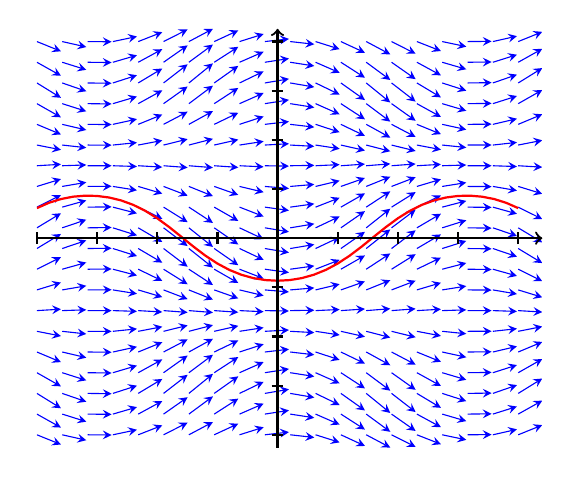
\begin{tikzpicture}
      \begin{axis}[
        axis line style={thick},
        tick style={thick, black},
        width=8cm,
        view={0}{90},
        %xmin=-4.2, xmax=4.7,
        %ymin=-4.5, ymax=4.5,
        axis lines=middle,
        axis line style={->},
        hide z axis=true,
        xtick distance=1,
        xticklabel=\empty,
        ytick distance=1,
        yticklabel=\empty,
        ]
        \addplot3[
        blue,
        quiver={
          u={1},
          v={sin(deg(x))*cos(deg(y))},
          scale arrows=0.4,
        },
        -stealth,
        samples=20,
        domain=-4:4,
        ] {0};
        \addplot[
        red,
        thick,
        ] table [row sep=crcr] {%
           -4	0.611526174567206 \\
           -3.8	0.719431140051444 \\
           -3.6	0.796217709609013 \\
           -3.4	0.843980278722318 \\
           -3.2	0.864663687744344 \\
           -3	0.859259346117522 \\
           -2.8	0.827499643465028 \\
           -2.6	0.767934909847919 \\
           -2.4	0.678425456833004 \\
           -2.2	0.557205813994516 \\
           -2	0.404630791166542 \\
           -1.8	0.225272223269531 \\
           -1.6	0.029195373874489 \\
           -1.4	-0.169154645466768 \\
           -1.2	-0.354678736552356 \\
           -1.0	-0.515783723872301 \\
           -0.8	-0.64634568928959 \\
           -0.6	-0.744988690358011 \\
           -0.4	-0.813067727063408 \\
           -0.2	-0.852753357122343 \\
           0	-0.865769483239659 \\
           0.2	-0.852753357122343 \\
           0.4	-0.813067727063407 \\
           0.6	-0.74498869035801 \\
           0.8	-0.646345689289588 \\
           1	-0.515783723872299 \\
           1.2	-0.354678736552353 \\
           1.4	-0.169154645466766 \\
           1.6	0.029195373874492 \\
           1.8	0.225272223269534 \\
           2	0.404630791166545 \\
           2.2	0.557205813994518 \\
           2.4	0.678425456833006 \\
           2.6	0.767934909847921 \\
           2.8	0.827499643465029 \\
           3	0.859259346117523 \\
           3.2	0.864663687744344 \\
           3.4	0.843980278722318 \\
           3.6	0.796217709609012 \\
           3.8	0.719431140051443 \\
           4	0.611526174567204 \\
         };
      \end{axis}
    \end{tikzpicture}
  \end{center}

Für b) $f(t,x)=x^2$
\begin{center}
    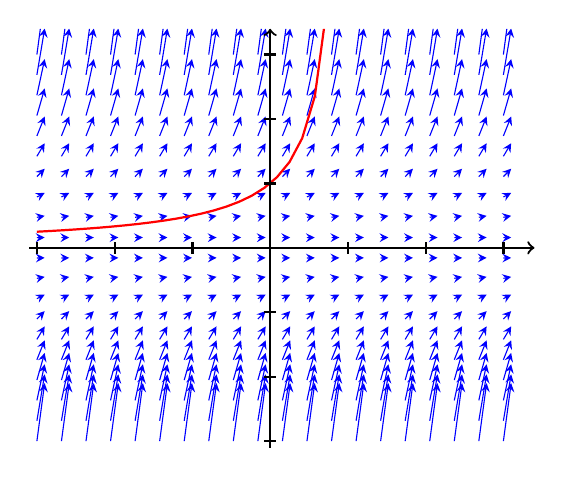
\begin{tikzpicture}
      \begin{axis}[
        axis line style={thick},
        tick style={thick, black},
        width=8cm,
        view={0}{90},
        xmin=-3.1, xmax=3.4,
        ymin=-3.1, ymax=3.4,
        axis lines=middle,
        axis line style={->},
        hide z axis=true,
        xtick distance=1,
        xticklabel=\empty,
        ytick distance=1,
        yticklabel=\empty,
        ]
        \addplot3[
        blue,
        quiver={
          u={1},
          v={y*y},
          scale arrows=0.1,
        },
        -stealth,
        samples=20,
        domain=-3:3,
        ] {0};
        \addplot[
        red,
        thick,
        domain=-3:0.90
        ] { 1/(1-\x) };
      \end{axis}
    \end{tikzpicture}
  \end{center}

Für c) $f(t,x)=-\frac{1}{\sqrt{x}}$

  \begin{center}
    \begin{tikzpicture}
      \begin{axis}[
        axis line style={thick},
        tick style={thick, black},
        width=5cm,
        view={0}{90},
        xmin=-0.3, xmax=2.1,
        ymin=-4.1, ymax=0.3,
        axis lines=middle,
        axis line style={->},
        hide z axis=true,
        xtick distance=1,
        xticklabel=\empty,
        ytick distance=1,
        yticklabel=\empty,
        ]
        \addplot[
        blue,
        domain=0.05:2,
        ] {-1/sqrt(x)};
      \path[pattern=north east lines, pattern color=red] (0,0) rectangle (-0.2,-4);
      \end{axis}
    \end{tikzpicture}
    \qquad\qquad
    \begin{tikzpicture}
      \begin{axis}[
        axis line style={thick},
        tick style={thick, black},
        width=5cm,
        view={0}{90},
        xmin=0, xmax=1.1,
        ymin=-0.3, ymax=1.1,
        axis lines=middle,
        axis line style={->},
        hide z axis=true,
        xtick distance=1,
        xticklabel=\empty,
        ytick distance=1,
        yticklabel=\empty,
        ]
        \addplot3[
        blue,
        quiver={
          u={1},
          v={-1/sqrt(y)},
          scale arrows=0.05,
        },
        -stealth,
        samples=10,
        domain=0.05:1,
        ] {0};
      \path[pattern=north east lines, pattern color=red] (0,0) rectangle (1.05,-1);
      \end{axis}
    \end{tikzpicture}
  \end{center}

\end{bsp}
Wann sind Lösungen bis an den Rand fortsetzbar? Die Antwort ist erstaunlich einfach!

Gegeben sei das AWP
\begin{equation*}
 	\dot{x}=f(t,x), \qquad x(t_0)=x_0.
\end{equation*}
\begin{satz}[Peano,1890]
	Sei $f \colon \Omega \subseteq \R \times \R^d \to \R^d$ stetig im zweiten Argument.
	Dann hat das AWP für alle $(t_0,x_0 ) \in \Omega$ mindestens eine Lösung.
	Jede Lösung lässt sich bis an den Rand von $\Omega$ fortsetzen.
\end{satz}
\begin{proof}[Skizze]
\begin{enumerate}
	\item Konstruiere eine numerische Approximation der vermuteten Lösung, mit Genauigkeitsparameter $h$.
	\item Die Folge dieser Approximationen für $h \to 0$ hat eine konvergente Teilfolge.
	\item Der Grenzwert dieser Teilfolge löst das AWP.
\end{enumerate}
\end{proof}

\subsection{Eindeutigkeit}

\begin{bsp}
	Betrachte $x' =\sqrt{\vert x \vert}$, $x(0)=0$. 
	Die Funktion $f(x)=\sqrt{\vert x \vert}$ ist stetig auf $\R$, es existiert also eine Lösung, z.B.: $x(t)=0$ für alle $t$. Eine weitere Lösung ist aber auch $x(t)=\frac{1}{4} t^2$ für $t>0$. Es kommt noch schlimmer:
	Für ein $c>0$, definiere
	\begin{equation*}
		\tilde{x}(t)\colonequals
		\begin{cases}
		0 & \text{falls}\ 0 \leq t \leq c \\
		\frac{1}{4} (t-c)^2 & \text{falls}\ c<t
			\end{cases}
	\end{equation*}
	Auch $\tilde{x}$ löst das Problem. Es gibt also unendlich viele Lösungen!
\end{bsp}

\begin{defi}
	Die Abbildung $f \in C(\Omega,\R^d)$ heißt auf $\Omega$ bzgl. $x$ lokal \begriff{Lipschitz-stetig}, wenn zu jedem $(t_0,x_0 ) \in \Omega$ ein offener Zylinder \begin{equation*}
		Z \colon (t_0-\tau,t_0+\tau ) \times B_{\rho} (x_0 ) \subset \Omega
	\end{equation*}
	existiert, in dem eine Lipschitzbedingung
	\begin{equation*}
	 \vert f(t,x)-f (t,\overline{x} ) \vert \leq L \vert x-\overline{x} \vert
	 \qquad
	 \forall (t,x),(t,\overline{x} ) \in Z
	\end{equation*}
	mit Konstante $L$ gilt.
\end{defi}

\begin{bem}
Falls $f(t,x)$ nach $x$ ableitbar ist, dann ist es auch bzgl.\ $x$ lokal Lipschitz-stetig.
\end{bem}

\begin{satz}[Picard--Lindelöf]
 Betrachte das Anfangswertproblem
 \begin{equation*}
  x' = f(t,x) \qquad x(t_0) = x_0
 \end{equation*}
 auf dem erweiterten Zustandsraum $\Omega \subset \R \times \R^d$ mit $(t_0, x_0) \in \Omega$.
 $f$ sei stetig und bzgl.\ $x$ lokal Lipschitz-stetig.

 Dann besitzt das AWP eine bis an den Rand von $\Omega$ fortgesetzte Lösung. Sie ist eindeutig bestimmt, d.h.\ Fortsetzung jeder weiteren Lösung.
\end{satz}
\begin{proof}[Skizze]
	Schreibe AWP als
	\begin{equation*}
		x(t)=x_0+\int_{t_0}^t f(s,x(s))\,ds
		\qquad
		\forall t \geq t_0
	\end{equation*}
	Konstruiere dafür eine Fixpunktiteration
	\begin{align*}
		\varphi_0 (t) & =x_0 \qquad \forall t \geq t_0 \\
		\varphi_{k+1} (t) & =x_0+\int_{t_0}^t f(s,\varphi_k(s))\,ds
		\qquad
		\tag{\text{Picard-Iteration}}
	\end{align*}
	Banachscher Fixpunktsatz: 
	\begin{enumerate}[nolistsep]
			\item Die Iteration konvergiert gegen einen Fixpunkt.
			\item Der Fixpunkt ist eindeutig.
		\end{enumerate}
	Der Fixpunkt löst das AWP.
\end{proof}


\section{Evolution und Phasenfluss}

Falls die Bedingungen des Satzes von Picard--Lindelöf gelten, so kann man eine elegante neue Notation einführen.

Sei $(t_0,x_0) \in \Omega$. Bezeichne mit $J_{\max} (t_0,x_0)$ das maximale Zeitintervall, auf dem eine Lösung des dazugehörigen AWPs existiert.
Zu jedem Anfangswert $(t_0,x_0 )$ gibt es eine eindeutige Lösung, d.h. zu jedem AW $(t_0,x_0 )$ ist der Wert $x(t)$ für alle $J_{\max} (t_0,x_0 )$ eindeutig bestimmt.

\begin{defi}
	Für alle $t_0,t \in J_{\max} (t_0,x_0 )$ heißt
	\begin{equation*}
		\Phi^{t,t_0} \colon x_0 \mapsto x(t)
	\end{equation*}
	\begriff{Evolution} der Differentialgleichung $x' = f(t,x)$.
\end{defi}

Die Evolution einer Differentialgleichung ist wohldefiniert, weil das AWP für jedes $x_0$ eine eindeutige Lösung hat. Man kann also schreiben: $x(t) = \Phi^{t,t_0} x_0$.

Der Satz von Picard--Lindelöf erhält folgende schöne Form: \cite[Lemma~2.9]{deuflhard_bornemann:2008}

\begin{satz}[Picard--Lindelöf]
	Es mögen die Bedingungen des Satzes von Picard--Lindelöf gelten.
	Für alle $(t_0,x_0 ) \in \Omega$ gilt
	\begin{equation*}
		J_\text{max} (t_0,x_0)= J_\text{max} (t,\Phi^{t,t_0} x_0)
		\qquad
		\forall t \in J_\text{max} (t_0,x_0).
	\end{equation*}
	Außerdem
	\begin{enumerate}
		\item $\Phi^{t_0,t_0} x_0=x_0$
		\item $\Phi^{t,s} \Phi^{s,t_0} x_0 = \Phi^{t,t_0} x_0$ für alle $t,s \in J_\text{max}(t_0, x_0)$.
	\end{enumerate}
\end{satz}

Für autonome Gleichungen $x'=f(x)$ kann man die Abhängigkeit von $t_0$ weglassen (wähle immer $t_0=0$). Der Evolutionsoperator $\Phi^t x_0=x(t)$ heißt dann \enquote{Phasenfluss}.

Aus den zwei Eigenschaften des vorigen Satzes wird dann
\begin{enumerate}
	\item $\Phi^0 x_0=x_0$
	\item $\Phi^t \Phi^s x_0=\Phi^{t+s} x_0$ (damit auch $\Phi^{-t} \Phi^t x_0=\Phi^0 x_0=x_0$).
\end{enumerate}
Der Phasenfluss $\Phi$ hat also eine Gruppenstruktur.


\section{Explizite Einschrittverfahren für AWP}

\begin{aim}
	Finde eine numerische Approximation der Lösung $x \in C^1 ([t_0,T],\R^d)$ des AWPs
	\begin{equation*}
		x' = f(t,x),
		\qquad
		x(t_0)=x_0
	\end{equation*}
\end{aim}

\emph{Vorgehensweise.}
\begin{itemize}
	\item Unterteile das Intervall $[t_0,T ]$ durch $n+1$ Zeitpunkte
	\begin{equation}
		t_0<t_1<t_2<\ldots<t_n=T.
	\end{equation}
	Die Menge der Zeitpunkte heißt \begriff{Gitter} $\Delta \colonequals \lbrace t_0,t_1,\ldots,t_n \rbrace$
	\item \begriff{Schrittweite}: $\tau_j\colonequals t_{j+1}-t_j$ für $j=0,\ldots,n-1$
	\item Maximale Schrittweite: $\tau_{\Delta}=\max_{j=0,\ldots,n-1} \tau_j$
\end{itemize}

Wir suchen eine Gitterfunktion
\begin{equation*}
	x_{\Delta} \colon \Delta \to \R^d,
\end{equation*}
welche die Lösung des AWPs an den Gitterpunkten möglichst gut approximiert.

\begin{bem}
	Manchmal interpretieren wir so ein $x_\Delta$ auch als eine Funktion $[t_0, T] \to \R^d$, die die
	Werte an den Gitterpunkten linear interpoliert.
\end{bem}

\fbox{\textbf{Das explizite Euler-Verfahren}}
nach \textsc{L. Euler} (1786), auch Eulersches Polygonzugverfahren

\begin{center}
	\begin{overpic}[width=0.5\textwidth]{explicit-euler}
		\put(2,25){$x_0$}
		\put(23,3){$t_0$}
		\put(45,3){$t_1$}
		\put(67,3){$t_2$}
	\end{overpic}
\end{center}

\begin{enumerate}[leftmargin=*]
	\item $x_{\Delta} (t_0)=x_0$
	\item Für $t \in [t_j,t_{j+1} ]$:
	\begin{equation*}
			x_{\Delta} (t)=x_{\Delta} (t_j )+(t-t_j ) f (t_j,x_{\Delta} (t_j ) )
	\end{equation*}
	\item Insbesondere:
	\begin{equation*}
	x_{\Delta} (t_{j+1} )=x_{\Delta} (t_j )+\tau_j f (t_j,x_{\Delta} (t_j ) )
	\end{equation*}
\end{enumerate}

Keine Gleichungsysteme zu lösen $\longrightarrow$ das Verfahren ist explizit.

Beachte: Berechnung durch eine Zweiterm-Rekursion
\begin{enumerate}
	\item $x_{\Delta} (t_0 )=x_0$
	\item $x_{\Delta} (t_{j+1} )=\Psi^{t_{j+1},t_j} x_{\Delta} (t_j ), j=0,1,\ldots,n-1$
\end{enumerate}
 mit $\Psi$ unabhängig von $\Delta$.

Die Funktion $\Psi$ heißt \begriff{diskrete Evolution} des expliziten Euler-Verfahrens.

Unsere Hoffnung ist natürlich, dass für immer feinere Gitter (wenn also $\tau_{\Delta}$ immer kleiner wird) der Unterschied zwischen $x$ und $x_{\Delta}$ immer kleiner wird.


\section{Konsistenz}

Der Fehler der Lösung, also der Unterschied $x - x_\Delta$, besteht aus zwei Beiträgen:
\begin{itemize}
 \item Jeder einzelne Schritt produziert einen Fehler.
 \item Da man nach dem ersten Schritt immer von einem fehlerbehafteten Wert startet, bekommt
  man auch falsche Ableitungen $f$.
\end{itemize}

Mit \begriff{Konsistenz} bezeichnet man das \textit{lokale} Verhältnis zwischen der Evolution $\Phi$ und der diskreten Evolution $\Psi$.
\begin{defi}
	Eine diskrete Evolution $\Psi$ heißt konsistent, falls
	\begin{alignat*}{2}
		\Psi^{t,t} x & =x &\qquad & \text{für alle $(t,x) \in \Omega$}, \\
		%
		\frac{d}{d \tau} \Psi^{t+\tau,t} x \Big|_{\tau=0} & =f(x,t)
		&& \text{für alle $(t,x) \in \Omega$}.
	\end{alignat*}
\end{defi}

\begin{defi}
	Sei $(t,x) \in \Omega$. Die Differenz 
	\begin{equation*}
		\varepsilon (t,x,\tau)=\Phi^{t+\tau,t} x-\Psi^{t+\tau,t} x
	\end{equation*}
	heißt \begriff{Konsistenzfehler}\footnote{Prof. Fischer: lokaler Diskretisierungsfehler} von $\Psi$.
\end{defi}

Man kann konsistente Evolutionen einfach charakterisieren.

\begin{lemma}[{{\cite[Lemma~4.4]{deuflhard_bornemann:2008}}}]
	Die diskrete Evolution $\Psi^{t+\tau,t} x$ sei für jedes $(t,x) \in \Omega$ und hinreichend kleines $\tau$
	bzgl.\ $\tau$ stetig differenzierbar. Dann ist äquivalent:
	\begin{enumerate}
		\item $\Psi$ ist konsistent
		\item $\Psi$ hat die Darstellung
		\begin{equation*}
			\Psi^{t+\tau,t} x=x+\tau \psi (t,x,\tau )
		\end{equation*}
		$\psi$ heißt \begriff{Inkrementfunktion}. $\psi$ ist stetig in $\tau = 0$, und
		\begin{equation*}
			\psi (t,x,0)=f(t,x).
		\end{equation*}
		
		\item Für den Konsistenzfehler gilt
		\begin{equation*}
			\varepsilon (t,x,\tau)=o (\tau),
			\qquad
			\tau \to 0
			\qquad
			(\text{also} \lim_{\tau \to 0} \frac{\varepsilon (\tau)}{\tau}=0 ).
		\end{equation*}
	\end{enumerate}
\end{lemma}

\begin{proof}
	Zunächst (1) $\Rightarrow$ (3):
	\begin{itemize}
		\item Taylor-Entwicklung von $\Phi$ um $\tau=0$
		\begin{align*}
			\Phi^{t+\tau,t} x & = \Phi^{t,t} x+\tau \cdot . \frac{d}{d \tau} \Phi^{t+\tau,t} x |_{\tau=0}+o(\tau) \\
			& = x+\tau \cdot f(t,x)+o(\tau)
		\end{align*}
		
		\item Ebenso für $\Psi$:
		\begin{equation} \label{eq:eqconsis}
			\Psi^{t+\tau,t} x=x+\tau \cdot f(t,x)+o(\tau)
		\end{equation}
		da $\Psi$ konsistent ist.
		
		\item Subtraktion zeigt (1) $\Rightarrow$ (3). Ebenso (3) $\Rightarrow$ (1)
	\end{itemize}
	Zu (2):
	\begin{itemize}
		\item \eqref{eq:eqconsis} bedeutet:
		\begin{align*}
			\Psi^{t+\tau,t} x & =x+\tau f(t,x) +\eta (t,x,\tau)
		\end{align*}
		mit einer Funktion $\eta$ für die $\lim_{\tau \to 0} \frac{\eta(\tau)}{\tau}=0$.
		
		\item Umformen ergibt
		\begin{align*}
			\frac{\Psi^{t+\tau,t} x-x}{\tau} & =f(t,x)+\frac{\eta (t,x,\tau)}{\tau}.
		\end{align*}
		Die Funktion
		\begin{align*}
			 \psi (t,x,\tau) \colonequals f(t,x)+\frac{\eta (t,x,\tau)}{\tau}
		\end{align*}
		ist also gerade die Inkrementfunktion aus (2).
		
		\item $\psi$ stetig und $\psi (t,x,0)=f(t,x)$, da $\eta \in o(\tau)$.
	\end{itemize}
\end{proof}

Das vorige Lemma beschreibt Äquivalenzen. Insbesondere gilt: Wenn sich $\Psi$ mit einer Inkrementfunktion schreiben lässt, so ist $\Psi$ konsistent.

\begin{bsp}
	Das explizite Euler-Verfahren
	\begin{equation*}
		\Psi^{t+\tau,t} x=x+ \tau f(t,x)=x+ \tau \psi (t,x,\tau)
	\end{equation*}
	ist konsistent.
\end{bsp}

Wir wollen eine \textit{quantitative} Version von Konsistenz.

\begin{defi}
	Eine diskrete Evolution $\Psi$ besitzt Konsistenzordnung $p$, wenn es eine Konstante $C>0$ unabhängig von $t$ und $x$ gibt, so dass
	\begin{equation*}
	 \varepsilon (t,x,\tau) \leq C \tau^{p+1}.
	\end{equation*}
\end{defi}

\begin{hinw}
	Ja, der Exponent ist wirklich $p+1$!
\end{hinw}

\begin{bsp}[Konsistenzordnung des Euler-Verfahrens]
Das Euler-Verfahren ist
\begin{equation*}
	 \Psi^{t+\tau,t} x=x+\tau f(t,x).
\end{equation*}

Sei $f \in C^1 (\Omega )$. Für den Konsistenzfehler $\varepsilon (t,x,\tau)=\Phi^{t+\tau,t} x-x-\tau f(t,x)$ machen wir eine Taylor-Entwicklung von $\Phi^{t+\tau,t} x$ in $\tau=0$:
	\begin{itemize}
		\item Erste Ableitung von $\Phi$ nach $\tau$:
		\begin{align*}
		\frac{d}{d \tau} \Phi^{t+\tau,t} x & =f (t+\tau,\Phi^{t+\tau,t} x )
		\end{align*}
		Warum? Sei $x(t) = \Phi^{t,t_0} x_0$ die Lösung des AWPs. 
		Dann ist $\Phi^{t+\tau,t}x = x(t+\tau)$ und
		\begin{align*}
			\frac{d}{d \tau} \Phi^{t+\tau,t} x & = x'(t+\tau) = f(t+\tau,x(t+\tau)) \\
			& = f (t+\tau,\Phi^{t+\tau,t} x ).
		\end{align*}
		%
		\item Zweite Ableitung (Kettenregel)
		\begin{align*}
			\frac{d^2}{d \tau^2} \Phi^{t+\tau,t} x
			& =
			f_t \big(t+\tau,\Phi^{t+\tau,t} x \big)+f_x \big(t+\tau,\Phi^{t+\tau,t} x \big)
			\cdot \underbrace{\frac{d}{d \tau} \Phi^{t+\tau,t} x}_{=f (t+\tau,\Phi^{t+\tau,t}x)}
		\end{align*}
		
		\item Taylor-Entwicklung um $\tau=0$:
		\begin{align*}
			\Phi^{t+\tau,t} x
			& = \Phi^{t+0,t} x+ \tau \cdot \frac{d}{d \tau} \Phi^{t+\tau,t} x \Big|_{\tau = 0}
			+\tau^2 \int_0^1 (1-\sigma ) \frac{d^2}{d \tau^2} \Phi^{t+\sigma\tau,t} x \,d \sigma \\
			& = x+\tau f(t,x)+\tau^2 \int_0^1 (1-\sigma) \Big[f_t \big(t+\sigma \tau,\Phi^{t+\sigma \tau,t} x \big) \\
			& \quad +f_x \big(t+\sigma \tau,\Phi^{t+\sigma \tau,t}x \big) f \big(t+\sigma \tau,\Phi^{t+\sigma \tau,t} x \big) \Big] d \sigma
		\end{align*}
	\end{itemize}
	Deshalb ist
	\begin{align*}
		\abs{\varepsilon (t,x,\tau)} & =\vert \Phi^{t+\tau,t} x-x-\tau f(t,x) \vert \\
		& = \tau^2 \vert \int_0^1 \ldots \,d \sigma \vert \\
		& \leq \tau^2 \frac{1}{2} \max_{(s,z) \in K} \vert f_t(s,z)+f_x(s,z)f(s,z) \vert
	\end{align*}
	Das Maximum existiert, denn es wird über eine kompakte Menge $K$ maximiert. Da wir nur an kleinen $\tau$ interessiert sind, können wir immer solch ein Kompaktum $K$, das alle relevanten $(t,x)$ enthält (siehe \cite[Beispiel~4.8]{deuflhard_bornemann:2008}).
	Die Konsistenzordnung ist also $1$.
\end{bsp}


\section{Konvergenz}

Konsistenz ist ein lokales Phänomen, d.h. es betrachtet den Fehler nur in der Nähe eines festen $t$. Wir betrachten jetzt, wie gut eine Lösung $x \in C^1 ([t_0,T])$ insgesamt approximiert wird und hoffen, dass für kleinere $\tau_{\Delta}=\max \tau_j$ die Approximation immer besser wird und das schnell!

\begin{defi}
	Der Vektor der Approximationsfehler auf dem Gitter $\Delta$
	\begin{equation*}
	 \varepsilon_{\Delta} \colon \Delta \to \R^d,
	 \qquad
	 \varepsilon_\Delta(t) = x(t)-x_{\Delta}(t)
	\end{equation*}
	heißt \begriff{Gitterfehler}. Seine Norm
	\begin{equation*}
		\Vert \varepsilon_{\Delta} \Vert_{\infty}=\max_{t \in \Delta} \vert \varepsilon_{\Delta} (t) \vert
	\end{equation*}
	heißt \begriff{Diskretisierungsfehler}.
\end{defi}

\begin{defi}
	Zu jedem Gitter $\Delta$ auf $[t_0,T]$ sei eine Gitterfunktion $x_{\Delta}$ gegeben. Die Familie dieser Gitterfunktionen konvergiert mit Ordnung $p \in \N$ gegen $x \in C^1([t_0,T])$, falls eine Konstante $C>0$ existiert, so dass
	\begin{equation*}
		\norm{\varepsilon_{\Delta}}_\infty \leq C \tau_{\Delta}^p
	\end{equation*}
	für alle $\tau_{\Delta}$ klein genug.
\end{defi}

\emph{Alternative Notation:} $\norm{\varepsilon_\Delta}_\infty = \mathcal{O}(\tau^p_\Delta)$.

Konvergenz hängt eng mit dem Konsistenzfehler zusammen. Das ist praktisch: Der Konsistenzfehler lässt sich häufig direkt am Verfahren ablesen.


\begin{satz}[{{\cite[Satz~4.10]{deuflhard_bornemann:2008}}}]
	Sei $\psi$ lokal Lipschitz-stetig in $x$. Die diskrete Evolution sei konsistent mit Ordnung $p$, d.h.
	\begin{equation*}
		\varepsilon(t,x,\tau) \colonequals x(t+\tau)-\Psi^{t+\tau,t} x(t)=\mathcal{O} (\tau^{p+1}).
	\end{equation*}
	Dann definiert die diskrete Evolution $\Psi$ für alle Gitter $\Delta$ mit hinreichend kleiner Zeitschrittweite $\tau_{\Delta}$ eine Gitterfunktion $x_{\Delta}$ zum Anfangswert $x_\Delta(t_0) = x_0$.
	Die Familie dieser Gitterfunktionen konvergiert mit Ordnung $p$ gegen die Lösung $x$ des AWPs, d.h.
	\begin{equation*}
		\norm{\varepsilon_{\Delta}}_{\infty}
		\colonequals
		\max_{t \in \Delta} \vert x(t)-x_{\Delta} (t) \vert =\mathcal{O} (\tau_{\Delta}^p)
	\end{equation*}
\end{satz}

\begin{proof}
	\begin{itemize}[leftmargin=*]
		\item Sei $K \subset \Omega$ kompakte Umgebung des Graphen der Lösung $x$.
		%
		\item $\psi$ ist lokal Lipschitz-stetig in $x$, d.h.\ es gibt $\tau_K, \Lambda_K > 0$ so dass
		\begin{equation*}
			\abs{\psi (t,x,\tau )-\psi (t,\overline{x},\tau )} \leq \Lambda_K \abs{x-\overline{x}}
		\end{equation*}
		für alle $(t,x),(t,\overline{x}) \in K$ und $\tau \in [0,\tau_K]$.
		%
		\item Insbesondere ist dann $\Psi^{t+\tau,t} x$ für alle $(t,x) \in K,0 \leq \tau \leq \tau_K$ definiert.
		%
		\item Es gibt einen \enquote{Schlauch} der Dicke $2 \delta_K>0$ um die Lösung $x$, der in $K$ enthalten ist.
		Genauer: Es gibt ein $\delta_K > 0$ so dass für alle $t \in [t_0,T]$
		\begin{equation*}
			\text{Falls $\abs{y-x(t)} \leq \delta_K$, so folgt $(t,y) \in K$.}
		\end{equation*}
		%
		\item Sei $\Delta$ Gitter für $[t_0,T ]$ mit $\tau_{\Delta} \leq \tau_K$.
		%
		\item \textit{Setze voraus}, dass $x_\Delta$ existiert und
		\begin{equation*}
			\abs{\varepsilon_{\Delta} (t)}
			=
			\abs{x(t)-x_{\Delta} (t)} \leq \delta_K \qquad \forall t \in \Delta.
		\end{equation*}
		%
		\item Betrachte $\varepsilon_{\Delta}$ genauer.  Der Gitterfehler im Gitterpunkt $t_{j+1}$ besteht aus
		zwei Teilen:
		\begin{align*}
			\varepsilon_{\Delta} (t_{j+1}) & =x (t_{j+1})-x_{\Delta} (t_{j+1}) \\
			& = x (t_{j+1})-\Psi^{t_{j+1},t_j} x_{\Delta} (t_j) \\
			& = \underbrace{x(t_{j+1})-\Psi^{t_{j+1},t_j} x (t_j)}_{\text{Konsistenzfehler}}
			+\underbrace{\Psi^{t_{j+1},t_j} x (t_j)-\Psi^{t_{j+1},t_j} x_{\Delta} (t_j)}_{\equalscolon \varepsilon_j}.
		\end{align*}
		%
		\item $\varepsilon_j$ kann als Propagation des Fehlers $\varepsilon_{\Delta} (t_j)$
		durch $\Psi$ zum Zeitpunkt $t_{j+1}$ interpretiert werden.
		Denn: Angenommen, $\Psi x$ sei linear in $x$ (ist es nicht!). Dann wäre
		\begin{equation*}
			\varepsilon_j=\Psi^{t_{j+1},t_j} (x(t_j)-x_{\Delta} (t_j)) =\Psi^{t_{j+1},t_j} \varepsilon_{\Delta} (t_j).
		\end{equation*}
		
		(\textit{Achtung:} $\varepsilon_j$ beschreibt eine Größe zur Zeit $t_{j+1}$!)
		%
		\item Darstellung von $\varepsilon_j$ mit der Inkrementfunktion:
		\begin{equation*}
			\varepsilon_j
			=x (t_j)-x_\Delta (t_j)
			+\tau_j \Big[\psi (t_j,x(t_j),\tau_j)-\psi (t_j,x_\Delta (t_j),\tau_j) \Big]
		\end{equation*}
		%
		\item Lipschitz-Stetigkeit von $\psi$:
		\begin{align*}
			\abs{\varepsilon_j}
			\leq
			\abs{\varepsilon_{\Delta} (t_j)}+\tau_j \Lambda_K \abs{x (t_j)-x_\Delta (t_j)}
			=
			(1+\tau_j \Lambda_K ) \abs{\varepsilon_\Delta (t_j)}
		\end{align*}
	\end{itemize}
	
	Da wir die Abschätzung für alle $j$ machen können folgt:
	\begin{enumerate}
		\item $\abs{\varepsilon_\Delta (t_0)} =0$
		\item $\abs{\varepsilon_{\Delta} (t_{j+1})}
		\leq C \tau_j^{p+1}+(1+\tau_j \Lambda_K) \abs{\varepsilon_{\Delta} (t_j)}$
	\end{enumerate}
	\emph{Behauptung:} Daraus folgt
	\begin{equation}
		\label{inequa:ineqerr1}
		\abs{\varepsilon_\Delta (t)}
		\leq
		\tau_{\Delta}^p \frac{C}{\Lambda_K} (e^{\Lambda_K (t-t_0)}-1 )
	\end{equation}
	für alle $t \in \Delta$.
	
	Damit haben wir
	\begin{equation*}
		\norm{\varepsilon_\Delta}_\infty
		\le
		\tau_\Delta^p \frac{C}{\Lambda_K} \big( e^{\Lambda_K (T-t_0)} - 1 \big)
		=
		\mathcal{O}(\tau_\Delta^p).
	\end{equation*}
	Achtung: wir mussten \emph{voraussetzen}, dass $\norm{\varepsilon_\Delta}_\infty$ klein ist!
\end{proof}

\begin{proof}[Beweis der Behauptung~\eqref{inequa:ineqerr1}] Induktion:
	\begin{itemize}
		\item Die Behauptung stimmt für $j=0$.
		%
		\item Angenommen die Behauptung ist richtig für $j<n$. Dann folgt
		\begin{align*}
			\abs{ \varepsilon_{\Delta} (t_{j+1}) }
			& \leq C \underbrace{\tau_j^{p+1}}_{\leq \tau_{\Delta}^p \cdot \tau_j}+(1+\tau_j \Lambda_K) \tau_{\Delta}^p \frac{C}{\Lambda_K} (e^{\Lambda_K (t_j-t_0)} -1 ) \\
			& \leq \tau_{\Delta}^p \frac{C}{\Lambda_K} [ \tau_j \Lambda_K + (1+\tau_j \Lambda_K) (e^{\Lambda_K (t_j-t_0)}-1 ) ] \\
			& = \tau_{\Delta}^p \frac{C}{\Lambda_K} [(1+\tau_j \Lambda_K) e^{\Lambda_K (t_j-t_0)}-1 ].
		\end{align*}
		%
		\item Es gilt aber $1+\alpha \leq e^{\alpha}$, bzw.\ $1+\tau_j \Lambda_K \leq e^{\tau_j \Lambda_K}$, also
		\begin{equation*}
			(1+\tau_j \Lambda_K) e^{\Lambda_K (t_j-t_0)} \leq e^{\Lambda_k \tau_j} e^{\Lambda_k (t_j-t_0)}
			=
			e^{\Lambda_K (t_{j+1}-t_0)}
		\end{equation*}
	\end{itemize}
\end{proof}

Für die Profis hier noch die Argumentation, warum die Annahme dass $\norm{\varepsilon_\Delta}_\infty$
klein ist, weggelassen werden kann.
\begin{itemize}
	\item Bisher mussten wir voraussetzen, dass
	\begin{equation*}
		\abs{\varepsilon_{\Delta} (t)} \leq \delta_K
		\qquad \text{für alle $t \in \Delta$.}
	\end{equation*}
	Jetzt haben wir aber \eqref{inequa:ineqerr1}!  Damit zeigen wir, dass die Bedingung gilt, wenn $\tau_\Delta$ klein genug ist.
	
	\item Wähle $\tau_* > 0$ so klein dass
	\begin{equation*}
		\tau_*^p \frac{C}{\Lambda_K} (e^{\Lambda_K(T-t_0)}-1) \le \delta_K
		\qquad \text{und} \qquad
		\tau_* \le \tau_K.
	\end{equation*}
	
	\item Wähle ein Gitter $\Delta$ auf $[t_0,T]$ mit $\tau_\Delta \le \tau_*$.
	
	\item Zeige mit der gleichen Induktion wie oben für alle $j$ dass
	\begin{itemize}
		\item die Abschätzung
		\begin{equation*}
			\abs{\varepsilon_\Delta(t_j)}
			\le
			\tau_\Delta^p \frac{C}{\Lambda_K} (e^{\Lambda_K(t_j-t_0)}-1) \le \delta_K
		\end{equation*}
		gilt, und deshalb
		\item $x_\Delta(t_{j+1})$ existiert.
	\end{itemize}
\end{itemize}
	
	
\begin{bsp}[Explizites Euler-Verfahren]
	$x_{j+1}=x_j+\tau_j f (t_j,x_j)$
	
	Das Verfahren hat Konsistenzordnung $1$ (der lokale Fehler verhält sich wie $\tau_{\Delta}$). Die Inkrementfunktion $\psi(t,x,\tau) = f(t,x)$ ist lokal Lipschitz-stetig in $x$.
	\begin{itemize}[leftmargin=*]
		\item[$\Rightarrow$] Verfahren konvergiert mit Ordnung $1$, d.h. $\Vert \varepsilon_{\Delta} \Vert_{\infty}=\mathcal{O} (\tau_{\Delta}^1 )$.
		\item[$\Rightarrow$] halber Fehler bedeutet doppelte Anzahl von Zeitschritten.
		\item[$\Rightarrow$] doppelte Anzahl von $f$-Auswertungen $\implies$ doppelter Aufwand
	\end{itemize}
\end{bsp}


\section{Explizite Runge--Kutta-Verfahren}

Können wir Verfahren mit einer höheren Konsistenzordnung konstruieren?

Wie lief der Beweis, dass das explizite Euler-Verfahren Konsistenzordnung $1$ hat?
\begin{itemize}[nolistsep]
	\item Konsistenzfehler:
	\begin{equation*}
		\varepsilon (t,x,\tau ) = \Phi^{t+\tau,t} x-\Psi^{t+\tau,t} x = (\Phi^{t+\tau,t} x-x )-\tau \psi (t,x,\tau)
	\end{equation*}
	\item Entwickle den Term in Klammern
	\begin{align*}
		\Phi^{t+\tau,t} x-x = \tau f (t,x)+\mathcal{O} (\tau^2)
	\end{align*}
	\item Euler-Verfahren: $\psi (t,x,\tau )=f(t,x)$ eliminiert gerade den ersten Term \\
	$\Rightarrow$ Konsistenzfehler ist $\mathcal{O}(\tau^2)$
\end{itemize}


\subsection{Taylor-Verfahren}

\begin{idea}
	Berechne weiteren Term der Taylor-Reihe:
	\begin{equation*}
		\Phi^{t+\tau,t} x-x
		=
		\tau f(t,x)+\frac{\tau^2}{2} [\frac{df(t,x)}{dt}+\frac{df(t,x)}{dx} \cdot f(t,x) ]+\mathcal{O} (\tau^3)
	\end{equation*}
\end{idea}
 
Inkrementfunktion für ein Verfahren mit Ordnung $2$:
\begin{equation*}
	\psi^* = f(t,x)+\frac{\tau}{2} \Big[f_t(t,x)+f_x(t,x) \cdot f(t,x) \Big]
\end{equation*}

So konstruierte Verfahren heißen \begriff{Taylor-Verfahren}. Im Prinzip ist dies für jede Ordnung möglich, solange $f$ glatt genug ist. Dabei müssen Ableitungen von $f$ berechnet werden, was mittels Automatischem Differenzieren sogar automatisch geht -- de facto aber nur für Ableitungen niedriger Ordnung. Deshalb findet dies in der Praxis kaum Anwendung.

\subsection{Idee der Runge-Kutta-Verfahren}

\begin{aim}
	 Hohe Ordnung ohne Ableitungen von $f$
\end{aim}
\begin{idea}
	\begin{itemize}
		\item Hauptsatz der Integralrechnung:
		\begin{equation*}
			x \colon [t_0,T] \to \R^d \qquad \text{löst} \qquad x' =f(t,x),
		\end{equation*}
		also
		\begin{equation*}
			x(t+\tau) = x(t)+\int_0^\tau f (t+\sigma,x (t+\sigma) )\,d\sigma
		\end{equation*}
		bzw.
		\begin{equation*}
			\Phi^{t+\tau,t} x-x = \int_0^\tau f (t+\sigma, \Phi^{t+\sigma,t} x )\,d\sigma
		\end{equation*}
		
		\item Approximiere das Integral numerisch, z.B.\ mit der Mittelpunktsregel / 1-Punkt Gauß--Legendre:
		\begin{equation*}
			\int_0^{\tau} f \big(t+\sigma, \Phi^{t+\sigma,t} x \big)\,d\sigma
			=
			\tau f (t+\frac{\tau}{2},\Phi^{t+\frac{\tau}{2},t} x )+\mathcal{O} (\tau^3)
		\end{equation*}
		\item Beachte: auch hier ist der Fehler in $\mathcal{O}(\tau^3)$!
	\end{itemize}
\end{idea}

Wie berechnet man aber $\Phi^{t+\frac{\tau}{2},t} x$?
\begin{itemize}
	\item Auf den ersten Blick nicht einfacher zu berechnen als $\Phi^{t+\tau,t}x$.
	\item \emph{Glück}: $\Phi^{t+\frac{\tau}{2},t} x$ taucht in einem Term auf, der mit $\tau$
	multipliziert wird.
	\item Es reicht deshalb, $\Phi^{t+\frac{\tau}{2},t} x$ bis auf $\mathcal{O}(\tau^2)$
	zu berechnen.
	\item Das geht mit dem expliziten Euler-Verfahren:
	\begin{equation*}
		\Phi^{t+\frac{\tau}{2},t} x=x+\frac{\tau}{2} f(t,x)+\mathcal{O} (\tau^2)
	\end{equation*}
	\item Man erhält das \begriff{Verfahren von Runge}:
	\begin{equation*}
		\Psi^{t+\tau,t} x = x+\tau f \Big(t+\frac{\tau}{2},x+\frac{\tau}{2} f(t,x) \Big)
	\end{equation*}
	mit Konsistenzordnung $2$.
	\item Zwei Auswertungen von $f$ pro Gitterpunkt, gegenüber 4 Auswertungen (von $f$ oder seinen Ableitungen) beim entsprechenden Taylor-Verfahren.
\end{itemize}

Den Ansatz von Runge kann man verallgemeinern. Das war der Beitrag von Kutta 1901.

Das Verfahren von Runge können wir in drei Schritten zerlegen:
\begin{enumerate}
	\item $k_1\colonequals f(t,x)$
	\item $k_2\colonequals f (t+\frac{\tau}{2},x+\frac{\tau}{2} k_1 )$
	\item $\Psi^{t+\tau,t} x=x+\tau k_2$
\end{enumerate}
	
Allgemein hat man ein $s$-stufiges explizites Runge-Kutta-Verfahren:
\begin{enumerate}
	\item $\displaystyle k_i\colonequals f \bigg(t+c_i \tau,x+\tau \sum_{j=1}^{i-1} a_{ij}k_j \bigg)
	\quad \forall i=1,\ldots,s$
	\item $\displaystyle \Psi^{t+\tau,t} x=x+\tau \sum_{i=1}^s b_ik_i$.
\end{enumerate}

Die Größen $k_i=k_i (t,x,\tau )$ heißen \begriff{\emph}{Stufen} des Verfahrens.

Koeffizienten: 
\begin{align*}
	A & = 
	\begin{pmatrix}
		0 \\
		a_{21} & 0 \\
		\vdots & \ddots \\
		a_{s1} & a_{s2} & \ldots & a_{s,s-1} & 0
	\end{pmatrix} \in \R^{s \times s}
	b & = (b_1,\ldots,b_s) \\
	c & = (c_1,\ldots,c_s) \\
\end{align*}
Traditionell notiert man die Koeffizienten im Butcher-Schema:
\begin{center}
	\begin{tabular}{c|c}
		$c^T$ & $A$ \\ \hline
		 & $b$
	\end{tabular}
\end{center}

\begin{bsp}
	\begin{itemize}[leftmargin=*]
		\item explizites Euler-Verfahren 
		\begin{tabular}{c|c}
			$0$ & $0$ \\ \hline
			& $1$
		\end{tabular}
		
		\item Verfahren von Runge 
		\begin{tabular}{c|cc}
			$0$ & $0$ &  \\
			$\frac{1}{2}$ & $\frac{1}{2}$ & $0$ \\ \hline
			& $0$ & $1$
		\end{tabular}
	\end{itemize}
\end{bsp}

\begin{itemize}
	\item Eine Funktionsauswertung pro Stufe
	\item $s + s + \frac{(s-1)s}{2}$ Parameter bei $s$ Stufen
\end{itemize}
Wie müssen die Koeffizienten gewählt werden, um eine möglichst hohe Konsistenzordnung zu erreichen?

\emph{Zuerst:} Konsistenz an sich (d.h. Konsistenz erster Ordnung)
\begin{itemize}
	\item Einschrittverfahren
	\begin{equation*}
		\Psi^{t+\tau,t} x=x+\tau \psi (t,x,\tau)
	\end{equation*}
	ist konsistent, wenn $\psi (t,x,0)=f(t,x)$ ist.
	
	\item Runge--Kutta-Verfahren:
	\begin{align*}
		k_i(t,x,0) 
		&= f \bigg(t+c_i \cdot 0,x+0 \cdot \sum_{j=1}^{i-1} a_{ij}k_j \bigg)
		= f(t,x)
		\\
		\psi (t,x,0) 
		&= \sum_{i=1}^s b_ik_i
		= f(t,x) \sum_{i=1}^s b_i
	\end{align*}
\end{itemize}

\begin{lemma}
	Ein explizites Runge--Kutta-Verfahren ist genau dann konsistent für alle $f \in C(\Omega,\R^d)$, wenn $\sum_{i=1}^s b_i = 1$.
\end{lemma}


\subsection{Autonomisierung}

Taylor- und Runge--Kutta-Verfahren brauchen $f \in C^p(\Omega,\R^d)$, also gleiche Glattheit in Zeit und Zustand. Wir wollen die Notation vereinfachen, und nur noch autonome Gleichungen betrachten. Ersetze
\begin{equation*}
  x' = f(t,x),
  \qquad
  x(t_0) = x_0
\end{equation*}
durch das erweiterte System
\begin{align*}
	\begin{pmatrix} x'(t) \\ s' (t) \end{pmatrix}
	= \begin{pmatrix} f (s(t),x(t)) \\ 1 \end{pmatrix} \qquad
	\begin{pmatrix} x(0) \\ s(0) \end{pmatrix}
	= \begin{pmatrix} x_0 \\ t_0 \end{pmatrix}.
\end{align*}
Beide Systeme haben die gleiche Lösung.
Runge--Kutta-Verfahren liefern aber möglicherweise \textit{unterschiedliche Lösungen} für die beiden Gleichungen und das ist natürlich hässlich!

\begin{lemma}
	Ein explizites Runge--Kutta-Verfahren ist genau dann invariant unter Autonomisierung, wenn es konsistent ist, und
	\begin{equation*}
		c_i=\sum_{j=1}^{i-1} a_{ij}
		\qquad
		\text{für $i=1,\dots,s$}
	\end{equation*}
	erfüllt.
\end{lemma}

Wir betrachten bis auf weiteres nur noch solche Runge--Kutta-Verfahren, und schreiben sie als $(b,A)$.
Betrachten wir nur noch autonome Probleme
\begin{equation*}
	x' = f(x)
	\qquad
	x(0) = x_0
\end{equation*}
 mit Phasenfluss $\Phi^t$, dann vereinfacht sich der diskrete Fluss $\Psi^{t+\tau,t}$ zu
\begin{equation*}
	\Psi^t x = x + \tau \psi(x,\tau).
\end{equation*}


\subsection{Konstruktion von Runge-Kutta-Verfahren}

Wir wollen ein Runge--Kutta-Verfahren $(b,A)$ der Ordnung $p$ konstruieren.
\begin{itemize}
	\item Wieviele Stufen brauche ich? $\to$ mindestens $p$ Stück
	\item Nach Autonomisierung sind noch $\frac{(s+1)s}{2}$ Koeffizienten zu bestimmen.
\end{itemize}

\begin{enumerate}[label=Schritt \arabic*, leftmargin=*]
	\item Aufstellung von Bedingungsgleichungen an die Koeffizienten, die die gewünschte Ordnung liefern.
	\item Lösen dieser Gleichungen.
\end{enumerate}

Wir behandeln den Fall $p=4$ und betrachten eine autonome Gleichung $x'=f(x)$ mit $f \in C^4(\Omega_0)$.

Ansatz: Entwickle den Konsistenzfehler $\varepsilon(x,\tau) = \Phi^\tau x - \Psi^\tau x$ in Taylor-Reihen bis auf $\mathcal{O}(\tau^5)$.
Konstruiere $\Psi$ so, dass die ersten $p$ Terme von $\varepsilon$ verschwinden.

\subsubsection{Taylor-Entwicklung des Phasenflusses \texorpdfstring{$\Phi^\tau$}{Phi^tau} nach \texorpdfstring{$\tau$}{tau}}

Vom Euler-Verfahren wissen wir schon dass
\begin{equation*}
	\Phi^{\tau} x=x+\tau f(x)+\frac{\tau^2}{2} f^{\prime} (x) \cdot f(x)+\mathcal{O} (\tau^3).
\end{equation*}

Wie bekommen wir die nächsthöhere Ordnung?

Trick:
\begin{equation*}
	\frac{d}{d \tau} \Phi^{\tau} x  =x'(\tau) = f(x(\tau),\tau) = f(\Phi^{\tau} x )
\end{equation*}
Einsetzen der Reihe für $\Phi^\tau$:
\begin{equation*}
	\frac{d}{d \tau} \Phi^{\tau} x = f \Big(x+\tau f(x)+\frac{\tau^2}{2} f'(x) \cdot f(x)+\mathcal{O}(\tau^3) \Big)
\end{equation*}
Taylor-Entwicklung davon:
\begin{align*}
	\frac{d}{d \tau} \Phi^{\tau} x
	& =
	f(x)+f'(x) \cdot \Big(\tau f(x)+\frac{\tau^2}{2} f'(x)f(x)+\mathcal{O} (\tau^3) \Big)
	+\frac{1}{2!}f^{\prime \prime}(x) (\tau f(x),\tau f(x))+\mathcal{O}(\tau^3) \\
	& =
	f+f^{\prime} f + \frac{\tau^2}{2} \Big(f'f'f + f''(f,f)\Big) +\mathcal{O}(\tau^3)
\end{align*}
Wir wollen aber eine Reihendarstellung von $\Phi^\tau x$.
Der Hauptsatz liefert:
\begin{align*}
	\Phi^{\tau} x
	& =
	x+\int_0^{\tau} \frac{d}{d \sigma} \Phi^{\sigma} x\,d\sigma \\
	& = x+\int_0^{\tau} \Big[f+\sigma f'f+\frac{\sigma^2}{2} (f'f'f+f^{\prime \prime} (f,f) )
	+\mathcal{O} (\sigma^3) \Big]\ d \sigma \\
	& =x+\tau f+\frac{\tau^2}{2} f'f+\frac{\tau^3}{3!} (f' f' f+f^{\prime \prime} (f,f) )+\mathcal{O}(\tau^4)
\end{align*}
d.h. wir bekommen eine Ordnung mehr. Führen wir das ganze nochmal aus:
\begin{align*}
	f(\Phi^{\tau} x)
	& =
	f+\tau f'f+\frac{\tau^2}{2} \big(f'f'f+f^{\prime \prime} (f,f)\big) \\
	&
	\quad +\frac{\tau^3}{3!} \Big[f^{\prime \prime \prime} (f,f,f)
	+3 f^{\prime \prime} (f'f,f)+f'f^{\prime \prime} (f,f)+f^{\prime}f^{\prime}f^{\prime}f \Big]
	+\mathcal{O}(\tau^4)
\end{align*}
Nochmalige Anwendung des Hauptsatzes liefert
\begin{align*}
	\Phi^{\tau} x
	& =
	x+\tau f+\frac{\tau^2}{2} f'f+\frac{\tau^3}{3!} \big(f'f'f+f^{\prime \prime} (f,f) \big) \\
	&
	\quad +\frac{\tau^4}{4!} \Big[f^{\prime \prime \prime} (f,f,f)
	+3 f^{\prime \prime} (f'f,f)+f'f^{\prime \prime} (f,f)+f'f'f'f \Big]+\mathcal{O}(\tau^5)
\end{align*}

\subsubsection{Taylorentwicklung des diskreten Flusses \texorpdfstring{$\Psi^\tau$}{Psi^tau}}

Ähnliches Spiel mit den Runge--Kutta Gleichungen
\begin{equation*}
	k_i \colonequals f \Big(x+\tau \sum_{j=1}^{i-1} a_{ij}k_j \Big)
	\qquad
	\text{für $i=1,\ldots,s$}.
\end{equation*}
$f$ ist stetig, also auf Kompakta beschränkt $\implies k_i$ beschränkt, $k_i=\mathcal{O}(1)$. Einsetzen: 
\begin{equation*}
	k_i
	=
	f \bigg(x+\tau \sum_{j=1}^{i-1} a_{ij} \mathcal{O}(1) \bigg)
	=
	f (x+\tau \mathcal{O}(1))
	=
	f(x+\mathcal{O} (\tau))
\end{equation*}
Taylor-Entwicklung um $x$:
\begin{equation*}
	k_i = f(x)+\mathcal{O}(\tau)
\end{equation*}
Einsetzen:
\begin{align*}
	k_i
	& =
	f \bigg(x+\tau \sum_{j=1}^{i-1} a_{ij} (f+\mathcal{O}(\tau)) \bigg)
	=
	f \big(x+\tau \sum_{j=1}^{i-1} a_{ij}f+\mathcal{O}(\tau^2) \big) \\
	&
	=f \big(x+\tau c_if+\mathcal{O} (\tau^2) \big)
	\qquad
	\text{mit $c_i = \sum_{j=1}^{i-1} a_{ij}$}.
\end{align*}
Taylor-Entwicklung:
\begin{equation*}
	k_i = f+\tau c_if'f + \mathcal{O}(\tau^2) \qquad \forall i=1,\ldots,s
\end{equation*}
Nochmal:
\begin{align*}
	k_i
	& =
	f \bigg(x+\tau \sum_{j=1}^{i-1} a_{ij} (f+\tau c_j f'f )+\mathcal{O} (\tau^3) \bigg) \\
	& =
	f+\tau c_i f'f+\tau^2 \sum_j a_{ij} c_j f'f'f+\frac{\tau^2}{2} c_i^2 f^{\prime \prime}(f,f)
	+\mathcal{O}(\tau^3)
\end{align*}
Nochmal:
\begin{align*}
	k_i
	& =
	f \bigg[ x + \tau c_i f + \tau^2 \sum_{j=1}^{i-1} a_{ij} c_j f' f
	+ \tau^3 \sum_{jk} a_{ij} a_{jk} c_k f'f'f \\
	& \qquad \qquad
	\frac{\tau^3}{2} \sum_j a_{ij} c_j^2 f''(f,f) + \mathcal{O}(\tau^4) \bigg]
	\\
	& =
	f+\tau c_i f'f+\tau^2 \sum_j a_{ij}c_j f'f'f+\frac{\tau^2}{2}c_i^2 f^{\prime \prime}(f,f) \\
	& \quad
	+\tau^3 \sum_{jk} a_{ij} a_{jk} c_k f'f'f'f + \frac{\tau^3}{2} \sum_j a_{ij} c_j^2 f' f''(f,f) \\
	& \quad
	+ \tau^3 \sum_{j} c_i a_{ij} c_j f''(f'f,f) + \frac{\tau^3}{6} c_i^3 f'''(f,f,f)
	+\mathcal{O}(\tau^4)
\end{align*}
Einsetzen in $\Psi^{\tau} x=x+\tau \sum_i b_ik_i$:
\begin{align*}
	\Psi^{\tau} x
	& =
	x+\tau \sum_{i=1}^s b_i f +\frac{\tau^2}{2} \bigg(2 \sum_i b_ic_i f'f \bigg) \\
	& \quad +
	\frac{\tau^3}{3!} \bigg[3 \sum_i b_ic_i^2 f'' (f,f)+6 \sum_{i,j} b_ia_{ij}c_j f'f'f \bigg] \\
	& \quad +
	\frac{\tau^4}{4!} \bigg[4 \sum_i b_ic_i^3 f''' (f,f,f)+24 \sum_{i,j} b_ic_ia_{ij}c_j f'' (f'f,f) \\
	& \quad
	+ 12 \sum_{i,j} b_ia_{ij}c_j^2 f' f'' (f,f) + 24 \sum_{i,j,k} b_ia_{ij}a_{jk}c_k f' f' f' f \bigg]
	+\mathcal{O}(\tau^5)
\end{align*}

Koeffizientenvergleich ergibt die Ordnungsbedingungen des folgenden Satzes:

\begin{satz}[{{\cite[Satz 4.18]{deuflhard_bornemann:2008}}}]
	Ein Runge--Kutta-Verfahren $(b,A)$ besitzt genau dann
	\begin{itemize}
		\item Konsistenzordnung $p=1$, falls $\sum\limits_{i=1}^s b_i=1$,
		\item Konsistenzordnung $p=2$, falls zusätzlich $\sum\limits_{i=1}^s b_ic_i=\frac{1}{2}$,
		\item Konsistenzordnung $p=3$, falls zusätzlich $\sum\limits_i b_ic_i^2=\frac{1}{3}$ und $\sum\limits_{i,j} b_ia_{ij}c_j=\frac{1}{6}$,
		\item Konsistenzordnung $4$, falls zusätzlich
		\begin{alignat*}{2}
			\sum_i b_ic_i^3 & =\frac{1}{4} & \qquad & \sum_{i,j} b_ic_ia_{ij}c_j=\frac{1}{8} \\
			\sum_{i,j} b_ia_{ij}c_j^2 & =\frac{1}{12} && \sum_{i,j,k} b_ia_{ij}a_{jk}c_k=\frac{1}{24}
		\end{alignat*}
		gelten.
	\end{itemize}
\end{satz}
(Eigentlich muss man noch zeigen, dass diese Bedingungen notwendig und nicht nur hinreichend sind.)

\subsubsection{Lösen der Gleichungen}

Wir wollen ein Verfahren vierter Ordnung.
\begin{itemize}
	\item Reichen $s=3$ Stufen? $\to$ Nein! 8 Gleichungen, aber nur $\frac{(s+1)s}{2}=6$ Unbekannte. Das Gleichungssystem ist überbestimmt und hat damit keine Lösung
	\item Reichen $s=4$ Stufen? Wir haben dann $\frac{(s+1)s}{2}=10$ Unbekannte, es könnte also gehen!
\end{itemize}

Unbekannte: $b_1,b_2,b_3,b_4,a_{21},a_{31},a_{32},a_{41},a_{42},a_{43}$
\begin{enumerate}
 \item \label{enum:rk4_gleichung_1} $b_1+b_2+b_3+b_4=1$
 \item \label{enum:rk4_gleichung_2} $b_1c_1+b_2c_2+b_3c_3+b_4c_4=\frac{1}{2}$
 \item \label{enum:rk4_gleichung_3} $b_2c_2^2+b_3c_3^2+b_4c_4^2=\frac{1}{3}$
 \item $b_3a_{32}c_2+b_4 (a_{42}c_2+a_{43}c_3 )=\frac{1}{6}$
 \item \label{enum:rk4_gleichung_5} $b_2c_2^3+b_3c_3^3+b_4c_4^3=\frac{1}{4}$
 \item $b_3c_3a_{32}c_2+b_4c_4 (a_{42}c_2+a_{43}c_3 )=\frac{1}{8}$
 \item $b_3 a_{32} c_2^2 + b_4 (a_{42} c_2^2 + a_{43} c_3^2) = \frac{1}{12}$
 \item $b_4 a_{43} a_{32} c_2 = \frac{1}{24}$
\end{enumerate}
Außerdem $c_i = \sum_{j} a_{ij}$ ($i=1,\dots,4$) insbesondere $c_1 = 0$.

Was nun? Gute Idee:
\begin{equation*}
	\int_0^1 1\,dx=1,
	\qquad
	\int_0^1 x\,dx=\frac{1}{2},
	\qquad
	\int_0^1 x^2\,dx=\frac{1}{3},
	\qquad
	\int_0^1 x^3 dx=\frac{1}{4}.
\end{equation*}
Approximiere die Integrale durch eine $4$-Punkt-Formel mit Stützstellen $c_1,c_2,c_3,c_4$ und Gewichten $b_1,b_2,b_3,b_4$. Falls die Formel exakt ist für kubische Polynome, erhält man die Gleichungen \ref{enum:rk4_gleichung_1},
\ref{enum:rk4_gleichung_2},\ref{enum:rk4_gleichung_3}, und \ref{enum:rk4_gleichung_5}.
Verwende die Simpson-Regel mit den Stützstellen $0,\frac{1}{2},1$ und Gewichten $\frac{1}{6},\frac{2}{3},\frac{1}{6}$. Verdoppeln wir den mittleren Punkt, erhalten wir
\begin{equation*}
	 c=(0,\frac{1}{2},\frac{1}{2},1 )
	 \qquad
	 b=(\frac{1}{6},\frac{1}{3},\frac{1}{3},\frac{1}{6} )
\end{equation*}
Damit kann man die fehlenden $a_{ij}$ bestimmen und erhält das klassische Runge-Kutta-Verfahren:
\begin{center}
	\begin{tabular}{c|cccc}
		$0$           &               &               &               &  \\
		$\frac{1}{2}$ & $\frac{1}{2}$ &               &               &  \\
		$\frac{1}{2}$ & $0$           & $\frac{1}{2}$ &               &  \\
		$1$           & $0$           & $0$           & $1$           &  \\ \hline
		              & $\frac{1}{6}$ & $\frac{1}{3}$ & $\frac{1}{3}$ & $\frac{1}{6}$ \\
	\end{tabular}
\end{center}

\hrulefill

%\section{Lineare Mehrschrittverfahren}
%
%\subsection{Einführung}
%Gegeben sei ein AWP
%\begin{equation*}
% x'(t) = f(t,x(t)),
% \qquad
% t \in [t_0,T],
% \qquad
% x(t_0)=x_0.
%\end{equation*}
%Approximation auf Gitter $\Delta=\lbrace t_0,\ldots,t_n\rbrace$ mit
%\begin{equation*}
% t_0<t_1<\ldots<t_n=T
%\end{equation*}
%durch Gitterfunktion $x_{\Delta}$ mit dem Ziel $x_{\Delta}(t_i) \approx x(t_i)$ für $i=1,\ldots,n$.
%
%\bigskip
%
%\emph{Bisher:} Einschrittverfahren
%\begin{itemize}
% \item Berechne $x_\Delta(t_{j+1})$ ausschließlich aus der Kenntnis des vorangegangenen Zustands $x_\Delta(t_j)$.
% \item Formalisierung: Diskrete Evolution
%  \begin{equation*}
%   x_\Delta(t_{j+1}) = \Psi^{t_{j+1},t_j} x_\Delta(t_j).
%  \end{equation*}
%\end{itemize}
%
%\medskip
%
%Eigenschaften der Einschrittverfahren:
%\begin{itemize}
% \item Konsistenztheorie eher schwierig
% \item Konvergenztheorie eher einfach
% \item Änderung der Zeitschrittweite jederzeit möglich.
% \item Verfahren hoher Ordnung sind teuer: Für Konsistenzordnung $p$ braucht man
%    (z.B.\ mit einem explizitien Runge--Kutta-Verfahren) mindestens $s \ge p$
%    Auswertungen der Funktion $f$.
%\end{itemize}
%
%
%\bigskip
%
%\paragraph{Idee der Mehrschrittverfahren:}
%Berechne den neuen Wert $x_\Delta(t_{j+1})$ aus den letzten $k$ Werten, also
%\begin{equation*}
% x_\Delta (t_{j-k+1}),\ldots,x_\Delta (t_j)
% \mapsto
% x_\Delta (t_{j+1}).
%\end{equation*}
%
%\medskip
%
%\emph{Vorteile:}
%\begin{itemize}
% \item nur eine einzige Auswertung von $f$ pro Schritt, für beliebig hohe Ordnung.
%\end{itemize}
%\emph{Nachteile:}
%\begin{itemize}
% \item Konvergenztheorie komplizierter,
% \item nicht so flexibel bei Änderungen der Schrittweite, schwierig auf nicht uniformen Gittern,
% \item $k$-Schritt-Verfahren benötigen neben Startwert $x_{\Delta}(t_0)$
%       noch $(k-1)$ zusätzliche Startwerte $x_\Delta(t_1),\ldots,x_\Delta (t_{k-1})$.
%\end{itemize}
%
%\subsection{Mehrschrittverfahren für äquidistante Gitter}
%
%Wir beschränken uns auf äquidistante (auch: uniforme) Gitter
%\begin{equation*}
% t_j=t_0+j \tau,\qquad j=0,1,\ldots,n
%\end{equation*}
%also
%\begin{equation*}
% \tau=\frac{T-t_0}{n}.
%\end{equation*}
%Dies ist nicht nur zur Bequemlichkeit.  Mehrschrittverfahren auf unregelmäßigen Gittern sind
%deutlich komplizierter!
%
%\bigskip
%
%\emph{Beispiel:} Die explizite Mittelpunktsregel
%\begin{itemize}
% \item Integriere die Differentialgleichung über $[t_{j-1},t_{j+1}]$:
% \begin{equation*}
%  x(t_{j+1})
%  =
%  x(t_{j-1}) + \int_{t_{j-1}}^{t_{j+1}} x'(\sigma)\,d\sigma
%  =
%  x(t_{j-1}) + \int_{t_{j-1}}^{t_{j+1}} f(\sigma,x(\sigma))\,d\sigma
% \end{equation*}
%
% \item Approximiere das Integral durch die Mittelpunktsregel
% \begin{equation*}
%  \int_{t_{j-1}}^{t_{j+1}} f(\sigma,x(\sigma))\,d\sigma
%  =
%  2\tau f(t_j,x(t_j)) + \mathcal{O}(\tau^3).
% \end{equation*}
%
% \item Mehrschrittverfahren
% \begin{equation*}
%  x_\Delta (t_{j+1} )=x_\Delta (t_{j-1} )+2 \tau f (t_j,x_\Delta (t_j ) ),\qquad j=1,\ldots,n-1
% \end{equation*}
%
% \item Verfahren ist explizit: Die gesuchte Größe $x_\Delta(t_{j+1})$ taucht nur links des
%  Gleichheitszeichens auf.
%
% \item Fehler der Integralapproximation ist $\mathcal{O}(\tau^3)$ (für $f$ hinreichend glatt).
%  Wir vermuten deshalb Konsistenzordnung $p=2$.
%\end{itemize}
%
%\bigskip
%
%Wie bekommt man höhere Konsistenzordnung?
%
%\medskip
%
%\emph{Idee:} Nimm genauere Quadraturformel!
%
%\medskip
%
%\emph{Beispiel:} Die Simpson-Regel
%\begin{equation*}
% \int_{t_{j-1}}^{t_{j+1}} f(\sigma,x(\sigma))\,d\sigma
% =
% \frac{\tau}{3} \Big[f (t_{j+1},x_(t_{j+1}))+4f (t_j,x(t_j))+f(t_{j-1},x(t_{j-1})) \Big]
% +
% \mathcal{O}(\tau^5)
%\end{equation*}
%
%\begin{itemize}
% \item Damit konstruiert man das Milne--Simpson-Verfahren
% \begin{equation*}
%  x_\Delta (t_{j+1})
%  =
%  x_\Delta (t_{j-1})
%  +
%  \frac{\tau}{3} \Big[f (t_{j+1},x_\Delta (t_{j+1}))+4f (t_j,x_\Delta (t_j))+f(t_{j-1},x_\Delta (t_{j-1})) \Big]
% \end{equation*}
%
% \item Konsistenzordnung $p=4$
%
% \item Dennoch nur \emph{eine} $f$-Auswertung pro Zeitschritt!
%
% \item Verfahren ist \emph{implizit}: Zur Bestimmung von $x_\Delta(t_{j+1})$ muss ein
%  Gleichungssystem gelöst werden.
%\end{itemize}
%
%\bigskip
%
%\paragraph{Allgemeine lineare $k$-Schritt-Verfahren:}
%\begin{itemize}
% \item Beide Beispiel-Verfahren sind linear in $f$.
% \item Definiere $f_\tau(t_i)$ als Abkürzung von $f(t_i,x_\Delta(t_i))$.
%\end{itemize}
%
%Definite das Verfahren
%\begin{multline}
%%\label{eq:allgemeines_msv}
% \alpha_k x_{\tau} (t_{j+k})+\alpha_{k-1} x_{\tau} (t_{j+k-1})+\ldots+\alpha_0 x_{\tau} (t_j) \\
% \label{equa:eqlMSV}
%  = \tau \Big[\beta_kf_{\tau} (t_{j+k})+\beta_{k-1}f_{\tau} (t_{j+k-1}) +\ldots+\beta_0f_{\tau} (t_j) \Big]
%\end{multline}
%mit $\abs{\alpha_0} + \abs{\beta_0} >0$ und $\alpha_k \neq 0$,
%(sonst ist es ein $(k-1)$-Schritt-Vefahren).
%\begin{itemize}
% \item Das Verfahren ist explizit, falls $\beta_k=0$. Ansonsten ist es implizit.
%\end{itemize}
%
%\bigskip
%
%Existiert eine eindeutige Gitterlösung?
%\begin{itemize}
% \item Explizites lMSV, also $\beta_k=0$ klar (sogar ohne Einschränkung an $\tau$).
%\end{itemize}
%
%\begin{lemma}
%Sei $\beta_k \neq 0$ und
%$f \ratio \R \times \R^d \to \R^d$ genüge der Lipschitz-Bedingung
%\begin{equation*}
% \norm{f(t,x)-f(t,\bar{x})} \leq L \norm{x-\bar{x}}
% \qquad
% \forall x,\bar{x} \in \R^d, t \in \R.
%\end{equation*}
%Dann existiert für $\tau <\frac{\abs{\alpha_k}}{\abs{\beta_k}L}$ zu beliebigen Startwerten
% $x_\Delta(t_0),\ldots,x_\Delta (t_{k-1})$ eine eindeutige Gitterfunktion $x_\Delta$ des lMSV.
%\end{lemma}
%\begin{proof}
%\begin{itemize}
% \item Löse \eqref{equa:eqlMSV} nach $x_\Delta(t_{j+k})$ auf:
%   \begin{equation*}
%    x_\Delta(t_{j+k}) = \tau \frac{\beta_k}{\alpha_k} f (t_{j+k},x_\Delta(t_{j+k}))+ \text{sonstige Terme}
%   \end{equation*}
%
% \item Dies ist eine Fixpunktgleichung.
%
% \item $\tau \frac{\beta_k}{\alpha_k}f$ ist Lipschitz-stetig mit Konstante $L^* = \tau \frac{\beta_k}{\alpha_k}L$
%
% \item Der Banachsche Fixpunktsatz liefert die Existenz eines eindeutigen Fixpunkts, wenn diese
%  Lipschitzkonstante $L^*$ kleiner $1$ ist, wenn also
%  \begin{equation*}
%   \tau <\frac{\abs{\alpha_k}}{\abs{\beta_k}L}.
%   %\qedhere
%  \end{equation*}
%\end{itemize}
%\end{proof}
%
%\bigskip
%\paragraph{Darstellung durch Polynome:}
%
%Zum Mehrschrittverfahren \eqref{equa:eqlMSV} definiere die Polynome
%\begin{align*}
% \rho   (\xi) & =\alpha_k \xi^k+\alpha_{k-1}\xi^{k-1}+\ldots+\alpha_0 \\
% \sigma (\xi) & =\beta_k \xi^k+\beta_{k-1}\xi^{k-1}+\ldots+\beta_0.
%\end{align*}
%
%\bigskip
%
%Zu den Beispielen:
%\begin{itemize}
% \item explizite Mittelpunktsregel: $\rho (\xi)=\xi^2-1$ und $\sigma (\xi)=2 \xi$
% \item Milne-Simpson: $\rho (\xi)=\xi^2-1$ und $\sigma (\xi)=\frac{1}{3} (\xi^2+4 \xi+1)$
%\end{itemize}
%
%\subsection{Konsistenz}
%
%Wir brauchen einen neuen Konsistenzbegriff.
%\begin{itemize}
% \item Beschreibt den Zusammenhang zwischen Differenzengleichung und Differentialgleichung.
%\end{itemize}
%
%\bigskip
%
%Plan:
%\begin{itemize}
% \item Ersetzen von $x_{\tau}$ durch die Funktion $x$, die die DGL erfüllt.
% \item Lokaler Diskretisierungsfehler $L(x,t,\tau)$ (hier wegen $f(t_j,x(t_j)) = x' (t_j)$)
% \begin{multline}
%   L(x,t,\tau)
%    \colonequals
%    \alpha_k x (t+k \tau )+\alpha_{k-1} x (t+(k-1) \tau )+\ldots+\alpha_0x(t) \\
%    \label{equa:eqL}
%    -\tau \Big[\beta_k x' (t+k \tau )+\beta_{k-1} x' (t+(k-1) \tau )+\ldots+\beta_0 x'(t) \Big]
% \end{multline}
%\end{itemize}
%\begin{defi}
%Das lMSV \eqref{equa:eqlMSV} besitzt die Konsistenzordnung $p$, wenn
%\begin{equation*}
% L (x,t,\tau )=\mathcal{O} (\tau^{p+1} )
%\end{equation*}
%für alle $x \in C^{\infty} ([t_0,T ],\R^d )$ und $\tau \to 0$ gleichmäßig für alle $t,\tau$ gilt.
%\end{defi}
%
%\bigskip
%
%Diese Definition ist eine Verallgemeinerung des bisherigen Konsistenzbegriffs.
%
%\medskip
%
%\emph{Beispiel:} Explizites Euler-Verfahren
%
%\begin{itemize}
% \item Lineares $1$-Schritt-Verfahren mit definierenden Polynomen $\rho (\xi )=\xi-1$ und $\sigma (\xi )=1$.
%
% \item Zugehöriger lokaler Diskretisierungsfehler
% \begin{align*}
%  L (x,t,\tau )
%  & =
%  x (t+\tau )-x(t)-\tau x'(t) \\
%  & =
%  x (t+\tau )- \big[ x(t) + \tau f(t,x(t)) \big] \\
%  & =
%  \Phi^{t+\tau,t} x - \Psi^{t+\tau,t} x.
% \end{align*}
%\end{itemize}
%
%
%
%\begin{lemma}
%Das lineare Mehrschrittverfahren~\eqref{equa:eqlMSV} hat genau dann die Konsistenzordnung $p$,
%wenn eine der folgenden äquivalenten Bedingungen erfüllt ist:
%\begin{enumerate}
% \item Für beliebige $x \in C^{p+1}([t_0,T],\R^d)$ gilt $L (x,t,\tau )=\mathcal{O} (\tau^{p+1} )$
%  gleichmäßig in allen zulässigen $t$ und $\tau$.
% \item \label{enum:lmsv_behandelt_polynome_exakt}
%  $L (Q,0,\tau )=0$ für alle Polynome $Q$ von Grad höchstens $p$
% \item $L (\exp,0,\tau )=\rho (e^{\tau} )-\tau \sigma (e^{\tau} )=\mathcal{O} (\tau^{p+1} )$
% \item \label{enum:lmsv_bestimmungsgleichungen}
%  Für alle $l=1,\ldots,p$ gilt
%  \begin{equation*}
%   \sum_{j=0}^k \alpha_j=0,
%   \qquad
%   \sum_{j=0}^k \alpha_jj^l=l \sum_{j=0}^k \beta_jj^{l-1}
%  \end{equation*}
%  (dabei gelte $0^0 = 1$).
%\end{enumerate}
%\end{lemma}
%
%\begin{proof}
%Wir zeigen $1) \implies 2) \implies 3) \implies 4) \implies 1)$.
%\begin{itemize}
% \item[$1) \implies 2)$:]
% \begin{itemize}
%  \item Für $Q \in \Pi_p$ ist $L (Q,0,\tau )$ ein Polynom in $\tau$.
%  \item Dessen Grad ist durch den von $Q$, also $p$, beschränkt.
%  \item Gleichzeitig ist $L(Q,0,\tau) = \mathcal{O}(\tau^{p+1})$.
%  \item Also ist $L (Q,0,\tau )=0$.
% \end{itemize}
% %
% \item $2) \implies 3)$
% \begin{equation*}
%  \exp (\tau )=Q (\tau )+\mathcal{O} (\tau^{p+1} )
% \end{equation*}
% mit $Q$ Taylorpolynom von $\exp$ an der Stelle $0$.
%
% Aus der Linearität von $L$ bzgl. des ersten Arguments folgt
% \begin{equation*}
%  L (\exp,0,\tau )=L (Q,0,\tau )+\mathcal{O} (\tau^{p+1} )
% \end{equation*}
% Wegen 2) ist $L (Q,0,\tau )=0$
% %
% \item $3) \implies 4)$
% Taylor-Entwicklung (nach $\tau$) an der Stelle $0$ liefert
% \begin{align*}
%  L (\exp,0,\tau)
%  & =
%  \sum_{l=0}^p \frac{1}{l!} \sum_{j=0}^k \alpha_jj^l \tau^l-\sum_{l=0}^{p-1} \frac{1}{l!} \sum_{j=0}^k \beta_jj^l \tau^{l+1}+\mathcal{O} (\tau^{p+1} ) \\
%  %
%  & =
%  \sum_{l=0}^p \frac{1}{l!} \sum_{j=0}^k \alpha_jj^l \tau^l
%     - \sum_{l=1}^p \frac{1}{(l-1)!} \sum_{j=0}^k \beta_j j^{l-1} \tau^l +\mathcal{O} (\tau^{p+1} )
% \end{align*}
% Koeffizientenvergleich bzgl. der $\tau$-Potenzen!
% %
% \item $4) \implies 1)$ Taylor-Entwicklung (nach $\tau$) an der Stelle $0$ liefert für $x \in C^{p+1}$:
% \begin{equation*}
%  L (x,t,\tau)
%  =
%  \sum_{l=0}^p \frac{1}{l!} \sum_{j=0}^k \alpha_jj^l \tau^l x^{(l)} (t)+\mathcal{O} (\tau^{p+1} )
%  -\tau [ \sum_{l=0}^{p-1} \frac{1}{l!} \sum_{j=0}^k \beta_jj^l \tau^l x^{(l+1)} (t)+ \mathcal{O}(\tau^p) ]
% \end{equation*}
% Koeffizientenvergleich liefert mit 4) ($=0$), also folgt die Aussage. %\qedhere
%\end{itemize}
%\end{proof}
%
%\bigskip
%
%\emph{Beispiel:} $p=0$.
%\begin{itemize}
% \item Wegen \ref{enum:lmsv_behandelt_polynome_exakt}) bedeutet das, dass konstante Funktionen exakt behandelt werden.
%
% \item D.h., das Anfangswertproblem
%  \begin{equation*}
%   x'=0, \qquad x(t_0) = x_0
%  \end{equation*}
%  wird exakt gelöst.
%
% \item Nach \ref{enum:lmsv_bestimmungsgleichungen}) ist die dazugehörige Bedingungsgleichung
% \begin{equation*}
%  \sum_{j=0}^k \alpha_j = 0,
%  \qquad \text{bzw.} \qquad
%  \rho(1) = 0.
% \end{equation*}
%\end{itemize}
%
%\medskip
%\emph{Beispiel:} $p=1$.
%\begin{itemize}
% \item Zusätzlich die Bedingungsgleichung
%  \begin{equation*}
%   \sum_{j=0}^k \alpha_j j = \sum_{j=0}^k \beta_k
%  \end{equation*}
%
% \item In Polynomform
%  \begin{equation*}
%   \rho'(1) = \sigma(1).
%  \end{equation*}
%\end{itemize}
%
%Diese Bedingungen entsprechen dem $\sum_{j=1}^s b_j = 1$ bei Runge--Kutta-Verfahren.
%
%\subsection{Stabilität}
%
%Bei Einschrittverfahren galt:
%\begin{itemize}
% \item Wenn ein Verfahren mit einer gewissen Ordnung konsistent ist, dann konvergiert es auch
%   mit dieser Ordnung.
%\end{itemize}
%So einfach ist es bei Mehrschrittverfahren leider nicht!
%
%\bigskip
%
%\begin{bsp}
%Betrachte das (bis auf Normierung $\alpha_k=1$) eindeutige explizite Zweischrittverfahren der Konsistenzordnung $p=3$
%\begin{equation}
% \label{equa:eqexD}
% \rho (\xi )=\xi^2+4 \xi-5,
% \qquad
% \sigma (\xi )=4 \xi +2.
%\end{equation}
%\begin{itemize}
% \item Anwendung auf
%  \begin{equation*}
%   x'(t)=0, \qquad x(0)=1
%  \end{equation*}
%  mit den Startwerten
%  \begin{equation*}
%  x_\Delta(0)=1, \qquad x_\Delta (\tau )=1+\tau \varepsilon.
%  \end{equation*}
%
% \item Man erhält die Gitterfunktion
%  \begin{equation*}
%   x_\Delta (n \tau )=1+\tau \varepsilon \frac{(1-(-5)^n )}{6}
%  \end{equation*}
%  (Beachte: $1$ und $-5$ sind gerade die Nullstellen von $\rho$!)
%
% \item Es folgt für alle $\varepsilon \neq 0$ dass
%  \begin{equation*}
%   \lim_{n \to \infty} \abs{ x_\Delta (n \tau ) } =\infty
%  \end{equation*}
% \item obwohl für den Startwert gilt, dass
%\begin{equation*}
% \lim_{\tau \to 0} x_\Delta (\tau )=1
%\end{equation*}
%und die exakte Lösung $x(t)=1$ beliebig glatt ist.
%\end{itemize}
%\end{bsp}
%
%
%Das heißt: keine Konvergenz, sogar ganz anderes Verhalten.
%\begin{itemize}
% \item Das Mehrschrittverfahren ist instabil.
% \item Es ist komplett unbenutzbar!
%\end{itemize}
%
%\bigskip
%
%\begin{defi}
%Ein lineares Mehrschrittverfahren heißt stabil (oder nullstabil oder D-stabil), wenn die lineare
%homogene Differenzengleichung
%\begin{equation*}
% \sum_{j=0}^k \alpha_jx_{\tau} (t_{j+k} )=0,
% \qquad
% k=0,1,\ldots
%\end{equation*}
%bei beliebigen Startwerten stabil ist.  Das wiederum heißt: Die Folge bleibt für alle Startwerte beschränkt.
%\end{defi}
%
%\medskip
%
%Beachte: Die homogene Differenzengleichung ist gerade das Mehrschrittverfahren, angewandt auf $x' = 0$.
%
%\medskip
%
%\begin{satz}[Dahlquistsche Wurzelbedingung]
%Ein lineares Mehrschrittverfahren ist genau dann stabil, wenn die Nullstellen $\xi$ von $\rho$ die Dahlquist'sche Wurzelbedingung
%erfüllen, d.h.
%\begin{itemize}
% \item $\vert \xi \vert \leq 1$,
% \item wenn $\vert \xi \vert =1$, dann ist $\xi$ einfache Nullstelle.
%\end{itemize}
%\end{satz}
%\begin{bsp}
%Für das lMSV \eqref{equa:eqexD} ist $\rho (\xi )=\xi^2+4 \xi-5=(\xi-1 ) (\xi+5 )$,
%d.h. dieses Verfahren ist nicht stabil.
%\end{bsp}
%
%\bigskip
%
%\begin{bsp}
% Für die explizite Mittelpunktsregel sowie für das Milne--Simpson-Verfahren ist $\rho(\xi) = \xi^2-1 = (\xi + 1)(\xi - 1)$.
% Beide sind also stabil.
%\end{bsp}
%
%\begin{bsp}
% Einschrittverfahren:
% \begin{itemize}
%  \item Sofern sie konsistent sind muss $\rho(1) = 0$, und deshalb $\rho(\xi) = \xi - 1$ gelten.
%  \item Alle konsistenten Einschrittverfahren sind deshalb automatisch stabil.
%  \item Beim Konvergenzbeweis für Einschrittverfahren mussten wir auf Stabilität deshalb gar nicht eingehen!
% \end{itemize}
%
%\end{bsp}
%
%\bigskip
%
%Wenn man sich die Bestimmungsgleichungen in \ref{enum:lmsv_bestimmungsgleichungen}) genauer anschaut, erkennt man:
%\begin{itemize}
% \item Es gibt $k$-Schritt-Verfahren mit Ordnung $2k$, aber keine mit höherer Ordnung.
% \item Es gibt explizite $k$-Schritt-Verfahren mit Ordnung $2k-1$, aber keine mit höherer Ordnung.
%\end{itemize}
%
%Wenn man sich auf \emph{stabile} Verfahren beschränkt verliert man in etwa die halbe Ordnung.
%
%
%
%\begin{satz}
% Die Konsistenzordnung $p$ eines stabilen linearen $k$-Schrittverfahrens unterliegt der Beschränkung
% \begin{enumerate}
%  \item $p \le k+2$, wenn $k$ gerade ist,
%  \item $p \le k+1$, wenn $k$ ungerade ist,
%  \item $p \le k$, wenn $\frac{\beta_k}{\alpha_k} \le 0$ ist, also insbesondere auch für explizite Verfahren.
% \end{enumerate}
%\end{satz}
%Diese Aussage nennt man die erste Dahlquistsche Schranke.
%
%Man kann zeigen dass sie scharf ist.
%
%\subsection{Konvergenz}
%
%\begin{definition}
%Sei $x \in C^1([t_0,T],\R^d)$ die Lösung eines Anfangswertproblems
%$x' = f(t,x)$, $x(t_0) = x_0$. Ein Mehrschrittverfahren \emph{konvergiert} gegen diese Lösung,
%wenn
%\begin{equation*}
% \lim_{\tau \to 0}  x_\Delta(t) = x(t)
% \qquad \text{für alle} \qquad
% t \in \Delta_\tau \cap [t_0,T]
%\end{equation*}
%gilt, sobald die Startwerte
%\begin{equation*}
%\lim_{\tau \to 0} x_{\Delta_\tau}(t_0 + j\tau) = x_0
%\qquad
%j = 0,\dots, k-1
%\end{equation*}
%erfüllen. Wenn ein lineares Mehrschrittverfahren für beliebige Anfangswertprobleme
%mit hinreichend glatter rechter Seite konvergiert, so heißt es konvergent.
%\end{definition}
%
%Das Phänomen aus dem obigen Beispiel ist von grundsätzlicher Natur, wie folgender Satz
%zeigt.
%\begin{satz}
%Ein konvergentes lineares Mehrschrittverfahren ist notwendigerweise stabil und konsistent,
%speziell gilt
%\begin{equation*}
% \rho'(1) = \sigma(1) \neq 0.
%\end{equation*}
%\end{satz}
%
%\bigskip
%
%Die Umkehrung gilt aber auch:
%\begin{satz}
% Ein stabiles und konsistentes lineares Mehrschrittverfahren ist konvergent.
%\end{satz}
%
%Dies ist ein gutes Beispiel dessen, was manche den Hauptsatz der Numerik nennen:
%\begin{quote}
%Konsistenz und Stabilität implizieren Konvergenz.
%\end{quote}
%
%Aussagen zur Konvergenzordnung sind natürlich auch möglich, gehen aber über den Rahmen
%dieser Vorlesung hinaus.
